\documentclass[10pt]{exam}
\usepackage[phy]{template-for-exam}
\usepackage{tikz}
\shadedsolutions
%\printanswers

\title{Energy \#4}
\author{Rohrbach}
\date{\today}

\begin{document}
\maketitle

\begin{questions}
  
\question
  A 1300-kg roller coaster starts at rest on the top of a 73-meter hill.  The track goes down to ground level before going up a second hill with a height of 45 meters.  There is no friction.

  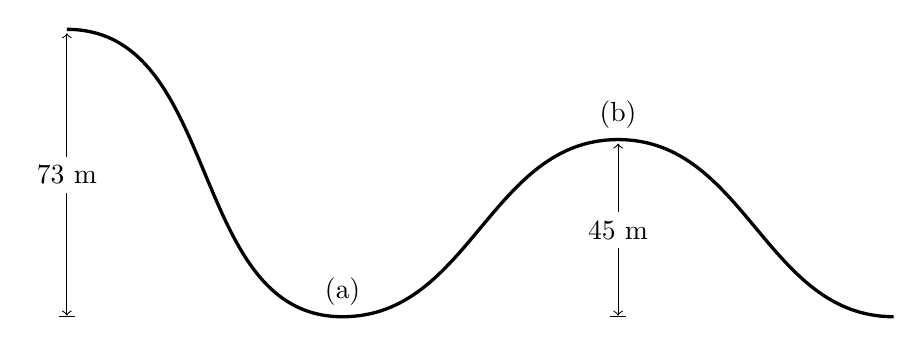
\begin{tikzpicture}[x=0.5cm, y=0.5cm]
    \def\xs{7}
    \draw[very thick] 
      (1*\xs,7.3) 
      to[in=180,out=0] (2*\xs,0) node[above] {(a)}
      to[in=180,out=0] (3*\xs,4.5) node[above] {(b)}
      to[in=180,out=0] (4*\xs,0);

    \draw[|<->] (\xs,0) -- (\xs,7.2) 
      node[midway,fill=white] {73 m};
    \draw[|<->] (3*\xs,0) -- (3*\xs,4.4) 
      node[midway,fill=white] {45 m};

  \end{tikzpicture}

  \begin{parts}
    \part
      How fast is the coaster travelling at the bottom of the first hill?
      
      \begin{solution}[\stretch{1}]
        \begin{align*}
          mgh_i           &= \frac{1}{2}mv_f^2 \\
          \SI{930020}{}   &= 650v_f^2 \\
          \SI{37.8}{\meter\per\second} &= v_f
        \end{align*}
      \end{solution}
   
    \part
      How fast is the coaster travelling at the top of the second hill?
      
      \begin{solution}[\stretch{1}]
        \begin{align*}
          mgh_i          &= \frac{1}{2}mv_f^2 + mgh_f \\
          \SI{930020}{}  &= 650v_f^2 + \SI{573300}{} \\
          \SI{23.4}{\meter\per\second} &= v_f
        \end{align*}
      \end{solution}
    
    \part
      Now, let's add friction to this problem.  With friction, the roller coaster does not make it to the top of the second hill; instead, it only reaches a height of 32 m before stopping.  How much work is done by friction?
      
      \begin{solution}[\stretch{1}]
        \begin{align*}
          mgh_i + W         &= mgh_f \\
          \SI{930020}{} + W &= \SI{407680}{} \\
          W                 &= \SI{-522340}{\joule}
        \end{align*}
      \end{solution}

  \end{parts}   


\pagebreak
  
\question
  A 2-kg block is kicked up a ramp with an initial speed of 5 m/s.

  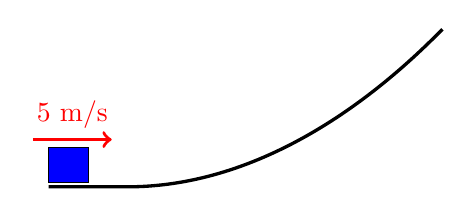
\begin{tikzpicture}
    \draw[very thick] (0,0) -- (1,0) parabola (5,2);
    \draw[fill=blue] (0,0.05) rectangle (0.5,0.5);
    \draw[red,->,very thick] (-.2,.6) 
      -- ++(1,0) node[midway, above] {5 m/s};
  \end{tikzpicture}

  \begin{parts}
    \part
      Assuming no friction, how high up the ramp would the block reach?
      
      \begin{solution}[\stretch{2}]
        \SI{1.28}{\meter}
      \end{solution}
    
    \part
      Instead, the block only makes it up 1.1 meters.  How much work was done by friction?
    
      \begin{solution}[\stretch{2}]
        \SI{3.44}{\joule}
      \end{solution}

  \end{parts}
  
\question
  Thomas the Tank Engine ($m = \SI{11500}{\kilo\gram}$) is barreling down the track at a speed of 45 m/s.  Batman's Batmobile has stalled at a level crossing 600 meters in front of him.  Thomas applies the brakes and comes to a stop just before running over the Batmobile.

  \begin{parts}

    \part
      How much work did Thomas's brakes do?
      
      \begin{solution}[\stretch{2}]
        \SI{-11643750}{\joule}
      \end{solution}

    \part
      What was the force of Thomas's brakes?
      
      \begin{solution}[\stretch{1}]
        \SI{-19406}{\newton}
      \end{solution}

  \end{parts}
  

\end{questions}

\end{document}